\q{22}{Get Off Your Phone}
\vskip .2in

A digital media company commissions a Berkeley Data Science club to conduct an analysis about how much time people spend on their phones. The club surveyed 500 people and collected the resulting data in the table \lsi+phones+ which has 5 columns: 
\begin{itemize}
    \item \lsi+Name+: The person's name
    \item \lsi+Model+: The type of phone the person has, an 'iPhone', 'Samsung Galaxy', 'Google Pixel', or 'Non-smartphone'
    \item \lsi+Screentime+: The average daily minutes that person spends on their phone
    \item \lsi+Data (MB/day)+: The average daily cell data usage of that person, in megabytes
    \item \lsi+Provider+: The person's cell phone carrier: 'AT\&T', 'Verizon', 'Sprint', or 'T-Mobile'
\end{itemize}

Here are the first 5 rows of the table, which has 500 rows total:
\begin{center}
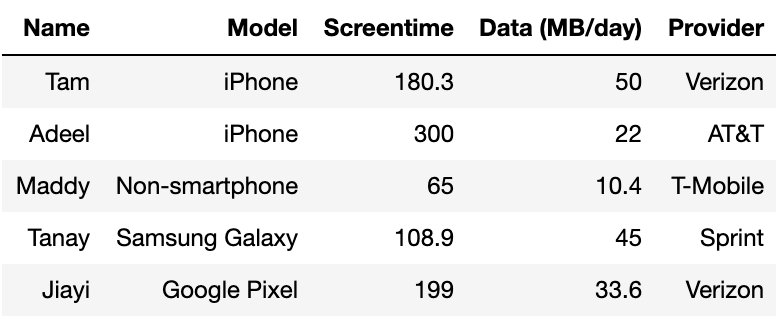
\includegraphics[scale=.9]{q1_phones}
\end{center}
\vskip .1in
\textbf{Fill in the blanks with Python expressions to compute the desired output.} ONLY use the blank lines provided. Some of the chained operations we might normally do in one line have been broken up into two or more lines,
storing intermediate results in tables or arrays. Do not write any code outside the blanks provided. The
expression in the last line should evaluate to the value described in the question.

\begin{enumerate}
\vskip 0.2in
\subq{2} Write code to assign \lsi+least_screen+ to the smallest value of daily screentime in the \lsi+phones+ table.
\vskip .2in
\solutionimage
{
\lstinline+least_screen =+\bklong\newline
}
{
\lstinline+least_screen = min(phones.column("Screentime"))+
}


\subq{3} Write code that assigns \lsi+num_iphones+ to the number of people with iPhones in the \lsi+phones+ table. 
\vskip .2in
\solutionimage
{{\lsi+iphones = phones.+\bkshort+("Model",+\bk+(+\bk+)+\nlvs}
\lstinline+num_iphones = iphones.+\bkmed
}
{
\lsi+iphones = phones.where("Model", are.equal_to("iPhone"))+\newline
\lstinline+num_iphones = iphones.num_rows+
}



\vskip .2in
\subq{4} Write code that assigns \lsi+high_provider+ to the cell phone provider of the person with the highest data usage. You can assume that data usages are unique in the \lsi+phones+ table.

\solutionimage
{
\vskip .2in
{\lsi+sorted = phones.+\bkshort+(+\bk+,+\bkmed+)+\nlvs}
{\lsi+high_provider = sorted.+\bkshort+.(+\bk+).+\bkshort+(+\bk+)+\nlvs}
}
{
\vskip .2in
\lsi+sorted = phones.sort("Data MB/day", descending=True)+\newline
\lstinline+high_provider = sorted.column("Provider").item(0)+
\vskip .4in
}




\subq{3} Write code that assigns \lsi+average+ to a table with two columns: one containing all of the phone models, and another containing the average screentime for each model.
\vskip .2in
\solutionimage
{
{\lsi+average = phones.+\bkshort+(+\bkshort+,+\bkshort+).select(+\bkshort+,+\bk+)+\nlvs}
}
{
\lsi+average = phones.group("Model", np.mean).select("Model", "Screentime mean")+
\vskip 0.2in
}


\subq{6} Later on in the project, a club member creates a table with information about cell phone providers and data costs. The \lsi+providers+ table has two columns:
\begin{itemize}
    \item \lsi+Company+: The name of the cell phone provider (“AT\&T”, “Verizon”, “Sprint”, or “T-Mobile”)
    \item \lsi+Price ($/MB)+: The price the company charges per megabyte of data used.
\end{itemize}
\begin{center}
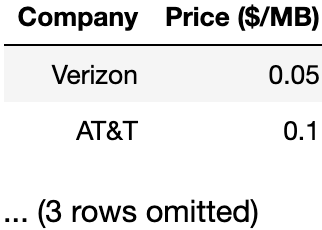
\includegraphics[scale=1]{q1_providers}
\end{center}
Write code to generate a table called \lsi+costs+ which contains two columns:
\begin{itemize}
    \item \lsi+Name+: The name of the person in the study
    \item \lsi+Monthly Cost+: The price the person has to pay for 30 days of data usage. Assume that every day, the person used the usage amount listed in the \lsi+phones+ table.
\end{itemize}
\vskip 0.2in
\solutionimage
{
{\lsi+all_info = phones.+\bkshort+(+\bk+,+\bk+,+\bk+)+\nlvs}
%{\lsi+daily_cost = +\bkshort+.+\bkshort+(+\bkshort+) * +\bkshort+.+\bkshort+(+\bkshort+)+\nlvs} %FIXME these lines r gonna be too short, probs need to split across lines
{\lsi+daily_usage = +\bkshort+.+\bk+(+\bk+)+\nlvs}
{\lsi+prices = +\bkshort+.+\bk+(+\bk+)+\nlvs}
{\lsi+daily_cost = daily_usage * prices +\nlvs}

{\lsi+monthly_cost = daily_cost * 30+\nlvs}
{\lsi+costs = Table().+\bk+(+\nlvs}
\hspace{1in}{\lsi+'Name', +\bkmed+,+\nlvs}
\hspace{1in}{\lsi+'Monthly Cost', +\bkmed+)+\nlvs}
}
{
{\lsi+all_info = phones.join("Provider",providers,"Company")+\nlvs}
%{\lsi+daily_cost = +\bkshort+.+\bkshort+(+\bkshort+) * +\bkshort+.+\bkshort+(+\bkshort+)+\nlvs} %FIXME these lines r gonna be too short, probs need to split across lines
{\lsi+daily_usage = all_info.column("Data MB/day")+\nlvs}
{\lsi+prices = all_info.column("Price $/MB")+\nlvs}
{\lsi+daily_cost = daily_usage * prices +\nlvs}

{\lsi+monthly_cost = daily_cost * 30+\nlvs}
{\lsi+costs = Table().with_columns(+\nlvs}
\hspace{1in}{\lsi+'Name', all_info.column("Name"),+\nlvs}
\hspace{1in}{\lsi+'Monthly Cost', monthly_cost)+\nlvs}
}

\vskip 2in

\subq{2} Write code so that \lsi+summary+ results in the following table:
\begin{center}
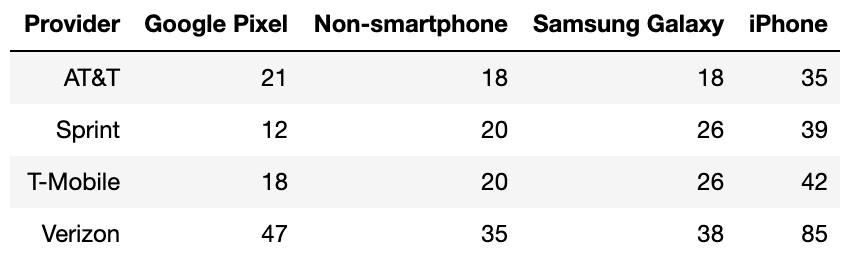
\includegraphics[scale=1]{q1_pivot}
\end{center}
The value in each cell represents the number of  people in the survey that had the corresponding phone/provider combination.
\vskip .1in
\solutionimage
{
\lstinline+summary = phones.+\bklong\newline
}
{
\lstinline+summary = phones.pivot("Model", "Provider")+
}

\vskip .3in
\subq{2} The following is a plot displaying the count of each phone model in the \lsi+phones+ table:
\begin{center}
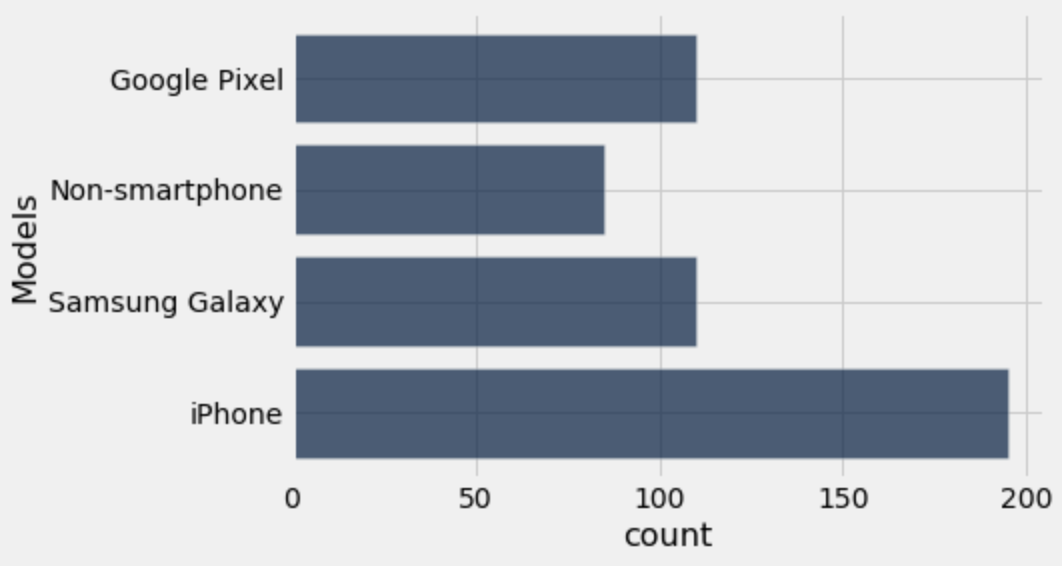
\includegraphics[scale=0.5]{q1_models}
\end{center}
Which line of code generated the above plot? 
\vskip .1in
{\bubble} \lsi+phones.barh('Model')+ \\
\solutionimage{\bubble}{\filledbubble}\lsi+phones.group('Model').barh('Model')+ \\
{\bubble} \lsi+phones.hist('Model')+\\
{\bubble} \lsi+phones.group('Model').hist('Model')+\\

\end{enumerate}
